Molecular structure originates from the underlying architecture of atoms, governed by quantum mechanical principles. Electrons are not treated as point particles following classical trajectories, but as wavefunctions—mathematical objects encoding the probability distribution of their position in space. The behaviour of an electron is determined not by Newtonian forces but by the solutions to the Schrödinger equation (Schrödinger, 1926), which defines discrete energy levels and corresponding spatial distributions.

The time-independent Schrödinger equation relates the system's total energy to its spatial properties: $\hat{H}\psi = E\psi$, where $\hat{H}$ is the Hamiltonian operator, $\psi$ is the electron wavefunction, and $E$ is the energy eigenvalue. These quantized solutions stand in sharp contrast to the continuous energy spectra predicted by classical mechanics and form the basis of modern atomic theory. Each solution defines an orbital, characterised by specific energy, shape, and nodal structure. In hydrogen, the $1\mathrm{s}$ orbital is spherically symmetric, while higher orbitals—$\mathrm{p}$, $\mathrm{d}$, and $\mathrm{f}$—exhibit directional lobes and angular nodes arising from quantum mechanical constraints.


\begin{figure}[htbp]
\centering
\pdftooltip{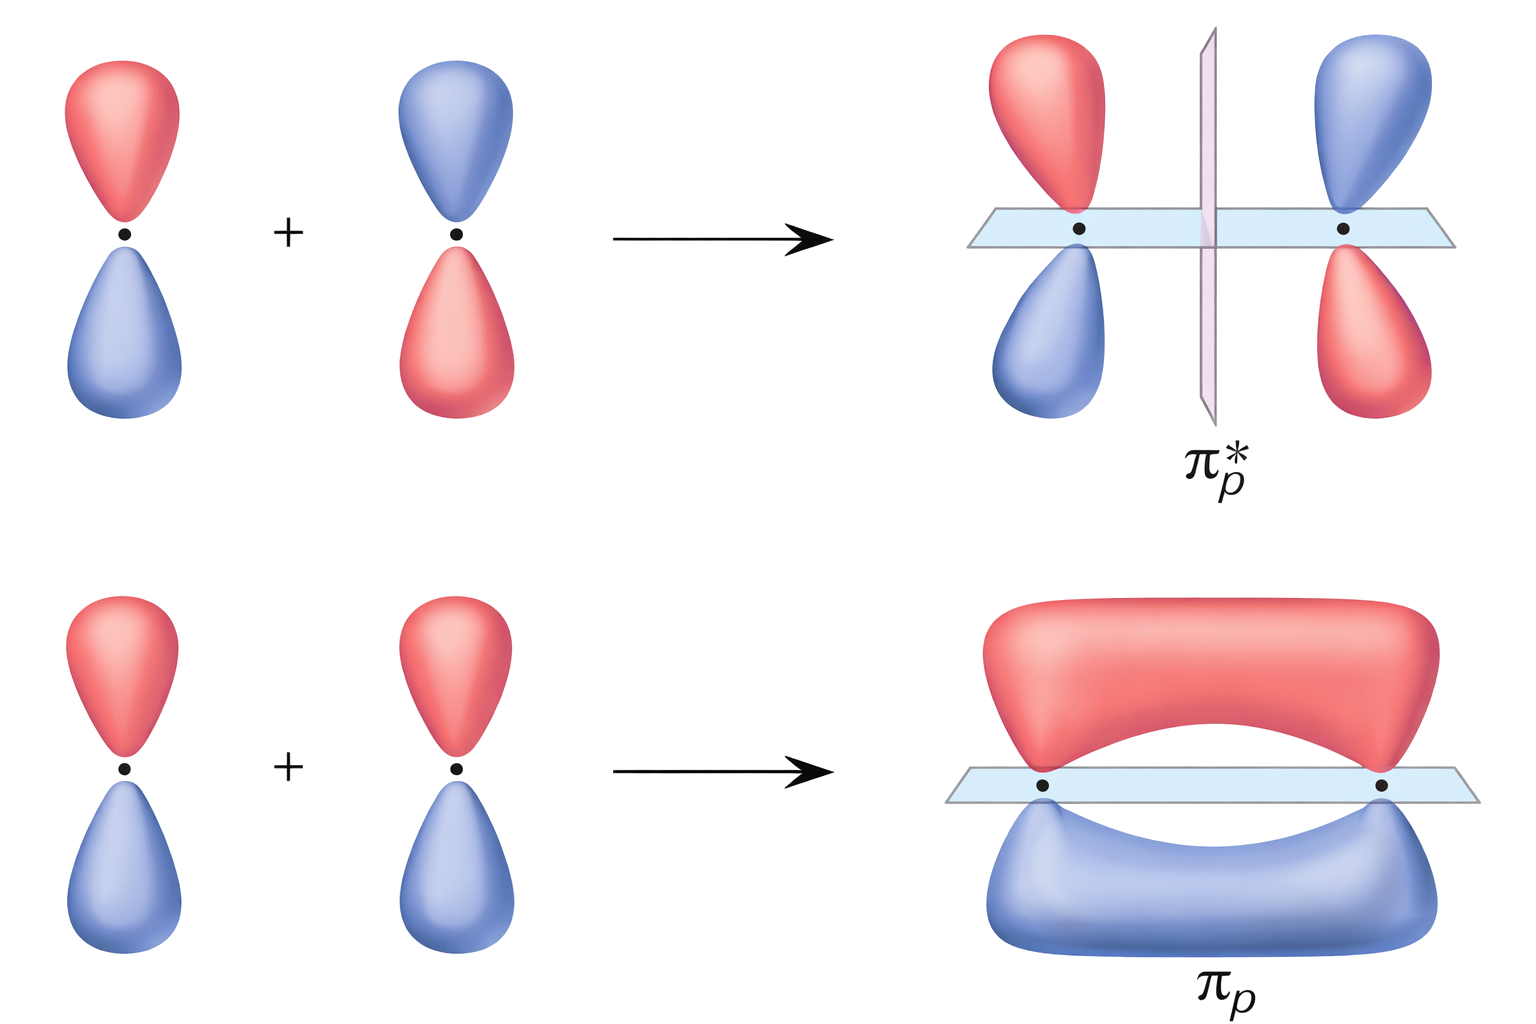
\includegraphics[width=0.6\textwidth]{46_WoodwardHoffmannRules/pMO_pi.png}}{Diagram showing the formation of bonding (pi) and antibonding (pi) molecular orbitals through lateral (side-on) overlap of two p atomic orbitals, with phase relationships indicated.}
\caption{Formation of $\pi$ and $\pi^*$ molecular orbitals from lateral overlap of $\mathrm{p}$ orbitals. Bonding $\pi_{\mathrm{p}}$ orbitals (bottom) feature electron density above and below the internuclear axis. Antibonding $\pi_{\mathrm{p}}^*$ orbitals (top) exhibit a nodal plane and out-of-phase lobes. Adapted from OpenStax Chemistry, Section 7.8: Molecular Orbital Theory. Licenced under CC BY 4.0.}
\label{fig:pi_p}
\end{figure}

When atoms bond to form molecules, their atomic orbitals combine into molecular orbitals that extend across multiple nuclei. Constructive interference between wavefunctions produces bonding orbitals, concentrating electron density between nuclei and stabilising the system. Destructive interference leads to antibonding orbitals, characterised by a nodal plane between nuclei and elevated energy. The occupation of these orbitals follows the Pauli exclusion principle (Pauli, 1925): electrons fill available molecular orbitals from lowest to highest energy, pairing spins where necessary. This filling determines the molecule’s electronic ground state and dictates its chemical reactivity.

\begin{figure}[htbp]
\centering
\pdftooltip{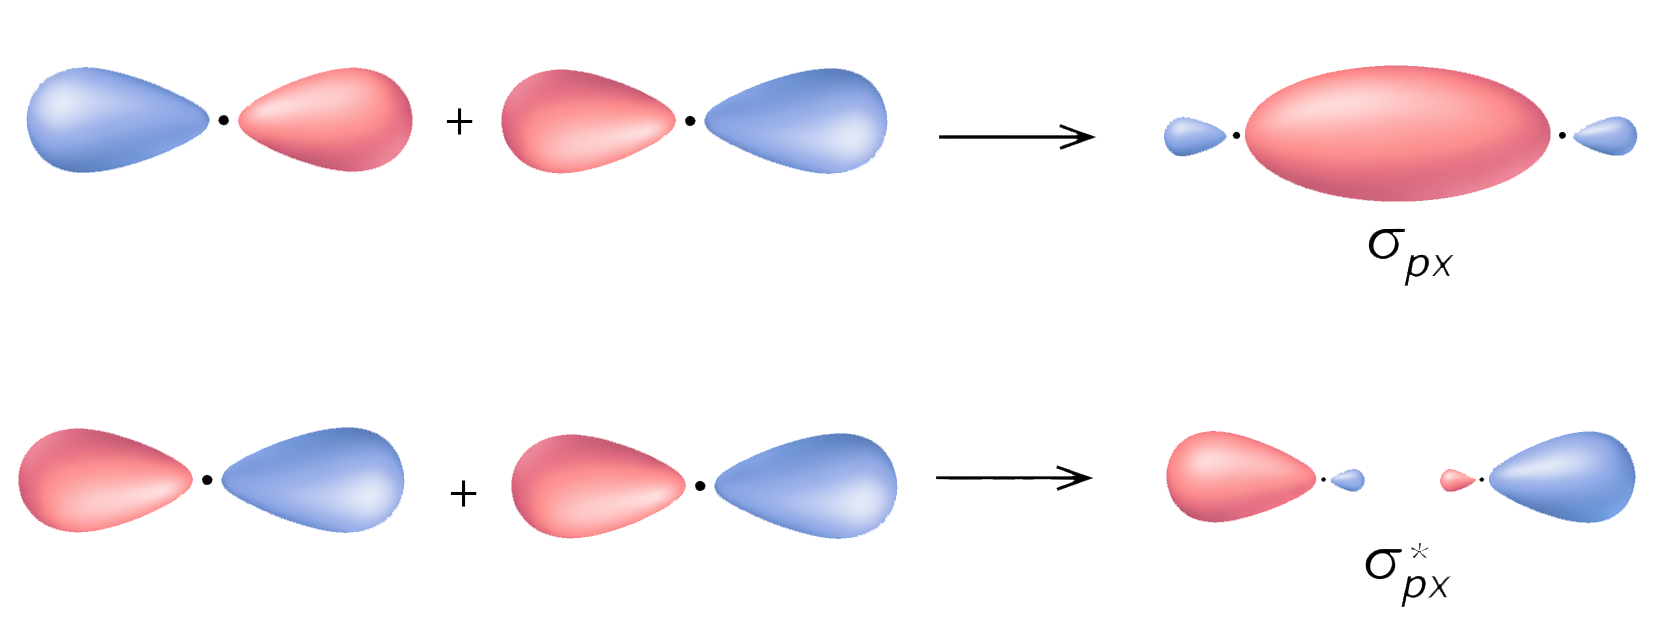
\includegraphics[width=0.7\textwidth]{46_WoodwardHoffmannRules/pMO_sigma.png}}{Diagram showing the formation of bonding (sigma) and antibonding (sigma) molecular orbitals through head-on overlap of two p atomic orbitals, with phase relationships indicated.}
\caption{Formation of $\sigma$ and $\sigma^*$ molecular orbitals from head-on overlap of two $\mathrm{p}_x$ atomic orbitals. Constructive interference (top) yields a bonding $\sigma_{\mathrm{p}_x}$ orbital. Destructive interference (bottom) yields an antibonding $\sigma_{\mathrm{p}_x}^*$ orbital. Adapted from OpenStax Chemistry, Section 7.8: Molecular Orbital Theory. Licenced under CC BY 4.0.}
\label{fig:sigma_px}
\end{figure}

Organic chemistry is dominated by molecules composed of carbon, hydrogen, oxygen, and nitrogen. Carbon’s tetravalency, enabled by $\mathrm{sp}^3$, $\mathrm{sp}^2$, and $\mathrm{sp}$ hybridisations of their $\mathrm{s}$ and $\mathrm{p}$ orbitals, allows the formation of stable $\sigma$ and $\pi$ bonds in chains, rings, and three-dimensional networks. $\pi$ bonds, arising from lateral overlap of unhybridized $\mathrm{p}$ orbitals, are more diffuse than $\sigma$ bonds and more sensitive to molecular geometry. In conjugated systems, $\pi$ bonds alternate with $\sigma$ bonds, allowing electron delocalisation across multiple atoms. This delocalisation lowers the system's energy and imparts distinctive electronic, optical, and chemical properties.

Conjugated $\pi$ systems underpin many organic processes, including pericyclic reactions. These reactions proceed concertedly: all bond-making and bond-breaking events occur simultaneously in a single kinetic step, without discrete intermediates. The hallmark of pericyclic reactions is cyclic electron flow, with electrons moving around a closed loop and the reaction passing through a highly ordered, often symmetric transition state. The feasibility and stereochemical outcome of these reactions depend critically on the phase relationships and symmetries of the participating molecular orbitals.

Molecular orbitals carry a property with no classical analogue: phase. Each orbital has regions of positive and negative sign, like the crests and troughs of a wave. When two orbitals overlap during a reaction, the outcome depends on whether their phases match. Constructive overlap—positive meeting positive—lowers the energy and drives bond formation. Destructive overlap—positive meeting negative—raises the energy and blocks it. Whether a reaction proceeds or not can hinge entirely on this sign, a purely mathematical property of the wavefunction.

The Woodward–Hoffmann rules (Woodward \& Hoffmann, 1965) formalised this into a predictive theory. The feasibility of any pericyclic reaction can be determined by tracking how the occupied molecular orbitals evolve along the reaction coordinate. If orbital symmetry is preserved continuously from reactants to products, the reaction is allowed. If symmetry is broken, the reaction is forbidden—no matter how thermodynamically favourable it might be.

The rules distinguish between thermal and photochemical activation. Under thermal conditions, reactions involve the ground electronic state, and the correlation of the highest occupied molecular orbitals (HOMOs) of reactants and products determines the pathway. Under photochemical conditions, excitation promotes an electron into a higher orbital, altering symmetry relationships. The relevant correlation then involves the frontier orbitals of the excited state. In both cases, the requirement is continuous, symmetry-allowed transformation of the electron configuration.

Electrocyclic reactions exemplify the application of the Woodward–Hoffmann rules. In the thermal ring closure of butadiene (four $\pi$ electrons), the terminal $\mathrm{p}$ orbitals must rotate conrotatorily—both twisting in the same direction—to preserve orbital symmetry and achieve constructive overlap. In contrast, the thermal ring closure of hexatriene (six $\pi$ electrons) proceeds through disrotatory motion, with terminal $\mathrm{p}$ orbitals rotating in opposite directions. Photochemical activation reverses these patterns: butadiene closes disrotatorily, and hexatriene closes conrotatorily.

The Diels–Alder reaction (Diels \& Alder, 1928) is the clearest demonstration. A conjugated diene (four $\pi$ electrons) and a dienophile (two $\pi$ electrons) combine in a single concerted step to form a six-membered ring—a [4+2] cycloaddition involving six $\pi$ electrons total. The reaction works thermally because the HOMO of the diene and the LUMO of the dienophile have matching phase at both ends simultaneously: both overlaps are constructive, so the transition state is stabilised. This reaction is a workhorse of organic synthesis—steroids, terpenes, alkaloids, and pharmaceutical intermediates are routinely built through Diels–Alder cycloadditions.

Now consider two ethylene molecules approaching face-to-face—a [2+2] cycloaddition with four $\pi$ electrons. The HOMO of one ethylene and the LUMO of the other have matching phase at one end but opposite phase at the other. One overlap is constructive, the other destructive. The net bonding interaction cancels, and the reaction faces a large energy barrier. Heat alone cannot drive it. Under ultraviolet irradiation, however, promoting an electron into the LUMO flips the phase relationship, making both overlaps constructive. The [2+2] cycloaddition becomes allowed photochemically—this is how cyclobutane rings are made. The same atoms, the same bonds to form, but the sign of a wavefunction determines whether the reaction needs a flame or a lamp.

Sigmatropic shifts extend the theory further. These reactions involve the migration of a $\sigma$-bonded group across a conjugated $\pi$ system. The symmetry of the transition state, visualised through correlation diagrams, dictates whether the shift is thermally allowed. For example, the [1,5]-hydride shift proceeds thermally because the orbital interactions preserve bonding symmetry throughout the migration.

The scope of the rules extends beyond synthetic chemistry into biological systems. In rhodopsin, the light-sensitive pigment of the retina, photoisomerisation of the retinal chromophore exemplifies a pericyclic process governed by symmetry. In its ground electronic state, thermal isomerisation is strongly disfavoured due to a high energy barrier and is extremely rare, preserving visual sensitivity. Upon photon absorption, the excited-state electronic configuration permits rapid, concerted isomerisation from the 11-cis to the all-trans configuration, triggering visual signal transduction.

Even pathological processes, such as the formation of toxic byproducts in age-related macular degeneration, follow orbital symmetry constraints. Under oxidative stress, reactive intermediates enable cyclisations that would otherwise be forbidden thermally.
\newpage
\begin{commentary}[Mathematical Abstraction as Physical Constraint]
The orbital symmetries that dictate reaction outcomes are not empirical regularities forced into a model. They are constraints embedded in the Schrödinger equation. When the mathematics of quantum mechanics was extended from atoms into molecular reaction pathways, it revealed new principles that had been invisible to empirical cataloguing. Symmetry conservation predicted which reactions would work, with what stereochemistry, before they were attempted. Few theories in chemistry have matched this kind of predictive reach from first principles.

This topic holds a personal significance for me. When I applied to a competitive excellence program at the Technion in Israel, I had almost no formal scientific education—my background was in yeshiva study. I was asked to give a lecture as part of the admissions process, and I chose the Woodward–Hoffmann rules. I could not claim deep technical fluency in organic chemistry, quantum mechanics, or group theory. But the subject sits at the intersection of all three, and presenting it allowed me to demonstrate a basic grasp of each—and, more importantly, a genuine curiosity about how they connect. It was the willingness to engage with an idea that crossed disciplinary boundaries, and the sense of wonder that comes from discovering a new connection between seemingly disparate fields, that ultimately led to my acceptance.
\end{commentary}

\inlineimage{0.35}{46_WoodwardHoffmannRules/MIRROR.png}{For some reason, mirrors flip the image left and right, but not up and down. \\ See the book \textbf{The Ambidextrous Universe} (1964) by M. Gardner.}{Cartoon demonstrating mirror reflection showing a figure and its reflection, with caption referencing the puzzle of why mirrors appear to flip left-right but not up-down, as discussed in Martin Gardne}